% -*- coding: utf-8; -*-

\chapter{Geração Baseada em Derivadas Médias}
\label{ch:my}
	Este capítulo descreve o método proposto nessa dissertação para gerar funções de transferência automáticas, baseado no trabalho de \textit{Kindlmann e Durkin}~\cite{gordon}, explicado no capítulo anterior.

\section{Detecção de Fronteiras}
\label{sec:my.deriv}
	Para eliminar o problema de deslocamento em $ h(v) $ é preciso repensar o modelo de \textit{Kindlmann e Durkin}~\cite{gordon} a fim de identificar a fronteira pela segunda derivada que não seja através de $ f''(x) = 0 $. Uma opção é utilizar o ponto de inflexão que ocorre quando $ f''(x) = 0 $. No entanto, como são encontrados três pontos de inflexão ao longo de $ f''(x) $, é preciso identificar aquele que ocorre quando $ f'(x) $ é máximo.
	
	Para encontrar o ponto de inflexão de uma função deve-se avaliar sua primeira e segunda derivadas. Na verdade, um ponto de inflexão é encontrado da mesma forma que a fronteira é identificada: um extremo local na primeira derivada e segunda derivada igual a zero. O que faz sentido, uma vez que segundo o modelo estipulado, o centro de uma fronteira é exatamente um ponto de inflexão. A Figura~\ref{fig:m_inflection} mostra $ f''(x) $ como $ D(x) $ e suas respectivas derivadas $ D'(x) $ e $ D''(x) $, onde os pontos de inflexão são indicados pelas retas tracejadas.
	
\begin{figure}[h]
	\centering
	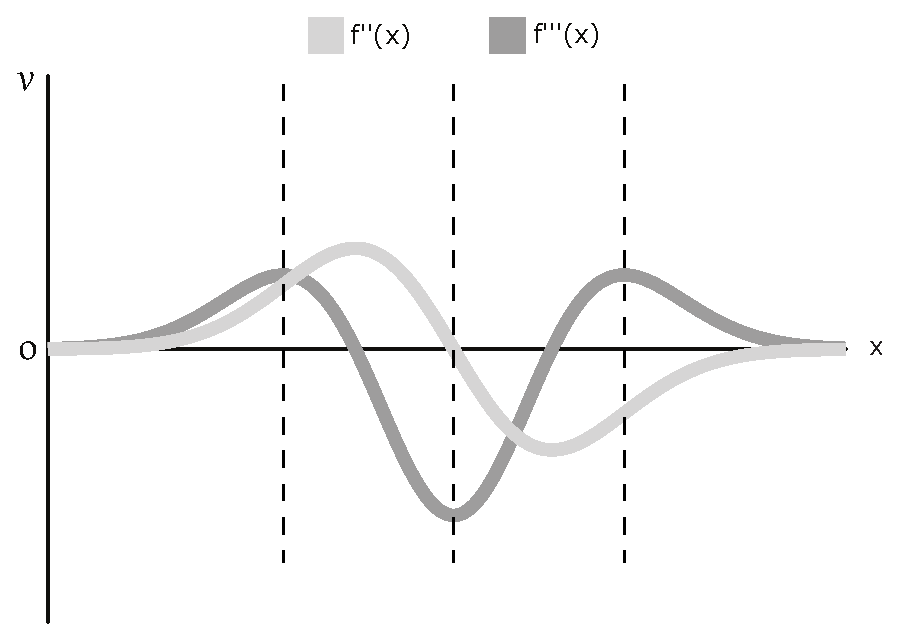
\includegraphics[width=0.7\textwidth]{images/m_inflection}
	\label{fig:m_inflection}
	%TODO
	\caption{Lalala...}
\end{figure}

	Vê-se que apenas um extremo de $ D'(x) $ é negativo. Essa informação é indiferente para encontrar os pontos de inflexão, mas é muito útil na detecção da fronteira, pois a posição do extremo negativo é justamente $ D(x) = 0 $, onde se encontra o centro da fronteira. Lembrando que $ D'(x) = f'''(x) $ percebe-se que $ f'''(x) $ pode ser utilizada para identificar uma fronteira, no lugar de $ f''(x) $, como mostra a Figura~\ref{fig:m_functions}.
	
\begin{figure}[h]
	\centering
	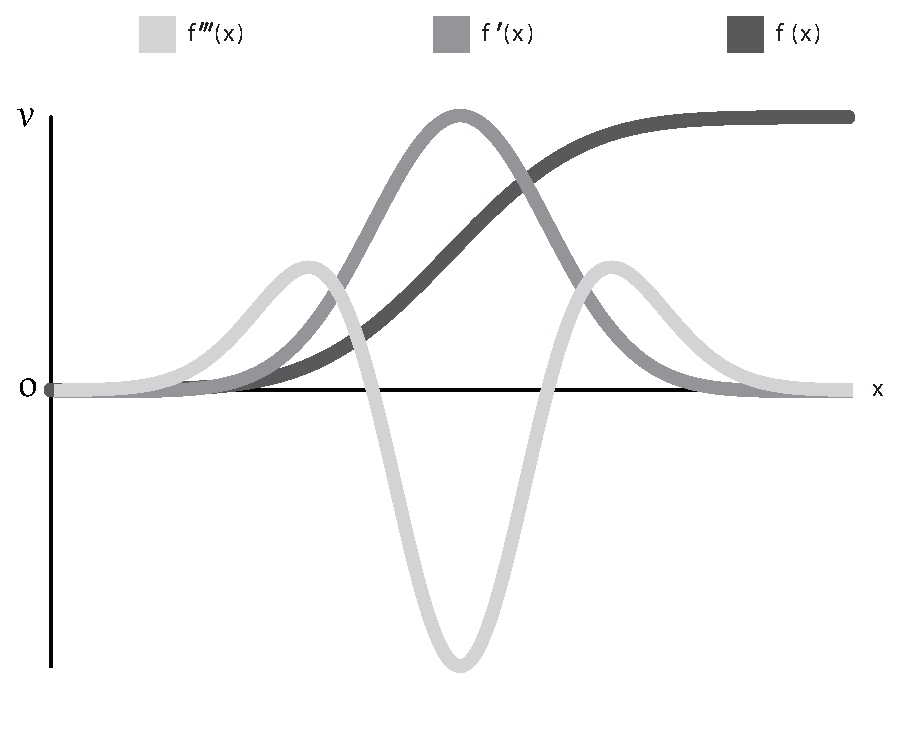
\includegraphics[width=0.7\textwidth]{images/m_functions}
	\label{fig:m_functions}
	%TODO
	\caption{Lalala...}
\end{figure}
	
	Ao optar pela terceira derivada, no lugar da segunda, elimina-se as chances de encontrar um $ v $ errado, devido ao deslocamento intrínseco às curvas médias. Contudo, perde-se a relação entre as derivadas e a distância à fronteira, definida na equação~\eqref{eq:x}. A partir da função $ f'''(x) $, exibida na equação~\eqref{eq:third}, pode-se encontrar uma nova expressão para $ \sigma $ e $ x $.
	\\
	
\begin{equation} \label{eq:third}
	t = f''(x) = -\frac{(x^{2} - \sigma^{2})(v_{max} - v_{min})}{\sigma^{5}\sqrt{2\pi}}\ e^{-\frac{x^{2}}{2\sigma^{2}}}
\end{equation} \\

\begin{equation} \label{eq:sigma3}
	\sigma^{2} = -\frac{f'(0)}{f'''(0)}
\end{equation} \\

\begin{equation} \label{eq:x3}
	x = \sigma^{2}\sqrt{\frac{f'''(x)}{f'(x)} + \frac{1}{\sigma^{2}}}
\end{equation} \\
    
\subsection{Malhas estruturadas}
\label{subsec:my.struct}
	Explicar malha estruturada...

\subsection{Malhas não estruturadas}
\label{subsec:my.nonstruct}
	Explicar malha não estruturada...

\section{Geração da função de transferência}
\label{sec:my.tf}
	Texto...